% Section content template for individual Educative lessons
% This file contains the actual content for a specific section
% Generated from Educative API section content

% Section: Detailed Design of Twitter
% Section ID: 6156135136755712
% Section Slug: detailed-design-of-twitter
% Generated: 2025-12-08T12:06:58.374767

\subsection{Storage system}\label{BOYQ86EbkY9OiCKgaPhER}
\\
\textbf{Storage} is one of the core components in every real-time system. Although we have a detailed chapter on storage systems, here, we'll focus on the storage system used by Twitter specifically. Twitter uses various storage models(A storage model represents a data store's essential physical aspects.) for different services to take full advantage of each model. We'll discuss each storage model and see how Twitter shifted from various databases, platforms, and tools to other ones and how Twitter benefits from all of these.
\\
The content in this lesson is primarily influenced by Twitter's technical blogs, though the analysis is ours.

\begin{itemize}
\item
\protect\phantomsection\label{UUoKohzK37JBjiLgC79RP}
\textbf{Google Cloud}: In Twitter, HDFS (Hadoop Distributed File System) consists of tens of thousands of servers to host over 300PB data. The data stores in HDFS are mostly compressed by the LZO (data compression algorithm) because LZO works efficiently in Hadoop. This data includes logs (client events, Tweet events, and timeline events), MySQL and Manhattan (discussed later) backups, ad targeting and analytics, user engagement predictions, social graph analysis, and so on. In 2018, Twitter decided to shift data from Hadoop clusters to the Google Cloud to better analyze and manage the data. This shift is named a \textbf{partly cloudy} strategy. Initially, they migrated Ad-hoc clusters (occasional analysis) and cold storage clusters (less accessed and less frequently used data), while the real-time and production Hadoop clusters remained. The big data is stored in the BigQuery (Google cloud service), a fully managed and highly scalable serverless data warehouse. Twitter uses the Presto (distributed SQL query engine) to access data from Google Cloud (BigQuery, Ad-hoc clusters, Google cloud storage, and so on).
\item
\protect\phantomsection\label{Yqjmm-2HrAzBWQZWUEvmb}
\textbf{Manhattan}: On Twitter, users were growing rapidly, and it needed a scalable solution to increase the throughput. Around 2010, Twitter used \textbf{Cassandra} (a distributed wide-column store) to replace MySQL but could not fully replace it due to some shortcomings in the Cassandra store. In April 2014, Twitter launched its own general-purpose real-time distributed key-value store, called Manhattan, and deprecated Cassandra. Manhattan stores the backend for Tweets, Twitter accounts, direct messages, and so on. Twitter runs several clusters depending on the use cases, such as smaller clusters for non-common or read-only and bigger for heavy read/write traffic (millions of QPS). Initially, Manhattan had also provided the time-series (view, like, and so on.) counters service that the MetricsDB now provides. Manhattan uses RocksDB as a storage engine responsible for storing and retrieving data within a particular node.
\end{itemize}

\begin{figure}[htbp]
 \centering
 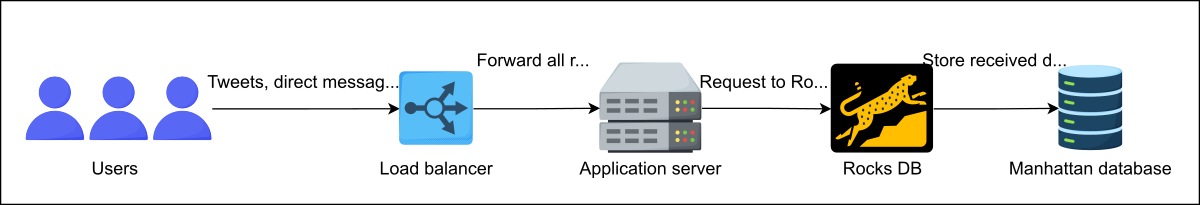
\includegraphics[width=0.5\textwidth]{Images/chapter_31/section_6156135136755712/5823666720210944.png}
 \caption{Twitter's data move to the Manhattan database}
\end{figure}

\begin{itemize}
\item
\protect\phantomsection\label{pLIVLz89dGRRMr0NWeiRO}
\textbf{Blobstore}: Around 2012, Twitter built the Blobstore storage system to store photos attached to Tweets. Now, it also stores videos, binary files, and other objects. After a specified period, the server checkpoints the in-memory data to the Blobstore as durable storage. We have a detailed chapter on the \href{https://www.educative.io/courses/grokking-the-system-design-interview/system-design-a-blob-store}{Blob Store}, which can help you understand what it is and how it works.
\item
\protect\phantomsection\label{dCMhYB2Ij3SztxPq3L8jE}
\textbf{SQL-based databases}: Twitter uses MySQL and PostgreSQL, where it needs strong consistency, ads exchange, and managing ads campaigns. Twitter also uses Vertica to query commonly aggregated datasets and Tableau dashboards. Around 2012, Twitter also built the Gizzard framework on top of MySQL for sharding, which is done by partitioning and replication. We have a detailed discussion on relational stores in our \href{https://www.educative.io/courses/grokking-the-system-design-interview/introduction-to-databases}{Databases} chapter.
\item
\protect\phantomsection\label{cWOAw4ZMVXYt9Twhwi-Ub}
\textbf{Kafka and Cloud dataflow}: Twitter evaluates around 400 billion real-time events and generates petabytes of data every day. For this, it processes events using Kafka on-premise and uses Google Dataflow jobs to handle deduping and real-time aggregation on Google Cloud. After aggregation, the results are stored for ad-hoc analysis to BigQuery (data warehouse) and the serving system to the Bigtable (NoSQL database). Twitter converts Kafka topics into Cloud Pub-sub topics using an event processor, which helps avoid data loss and provides more scalability. See the \href{https://www.educative.io/courses/grokking-the-system-design-interview/system-design-the-pub-sub-abstraction}{Pub-sub} chapter for a deep dive into this.
\end{itemize}

\begin{figure}[htbp]
 \centering
 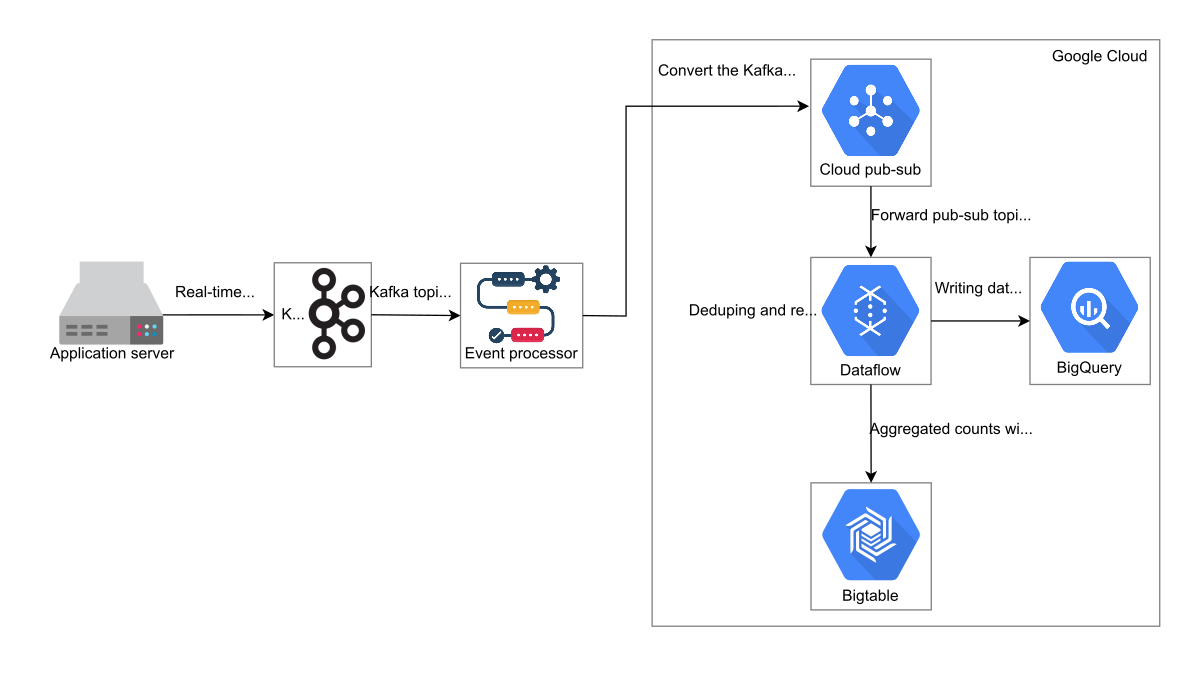
\includegraphics[width=0.5\textwidth]{Images/chapter_31/section_6156135136755712/4634658946678784.png}
 \caption{Real-time processing of billions of requests}
\end{figure}

\begin{itemize}
\item
\protect\phantomsection\label{OSPhWJM7XCPJpPqajDCLr}
\textbf{FlockDB}: A relationship refers to a user's followers, who the user follows, whose notifications the user has to receive, and so on. Twitter stores this relationship in the form of a graph. Twitter used FlockDB, a graph database tuned for huge adjacency lists, rapid reads and writes, and so on, along with graph-traversal operations. We have a chapter on \href{https://www.educative.io/courses/grokking-the-system-design-interview/introduction-to-databases}{Databases} and \href{https://www.educative.io/courses/grokking-the-system-design-interview/system-design-newsfeed-system}{Newsfeed} that discusses graph storage in detail.
\item
\protect\phantomsection\label{El8TV0z4c-_BjqgfcSLnz}
\textbf{Apache Lucene}: Twitter constructed a search service that indexes about a trillion records and responds to requests within 100 milliseconds. Around 2019, Twitter's search engine had an indexing latency (time to index the new tweets) of roughly 15 seconds. Twitter uses Apache Lucene for real-time search, which uses an inverted index(The inverted index is a data structure like a hashmap that directs the system from a word to a document or database table.). Twitter stores a real-time index (recent Tweets during the past week) in RAM for low latency and quick updates. The full index is a hundred times larger than the real-time index. However, Twitter performs batch processing for the full indexes. See the \href{https://www.educative.io/courses/grokking-the-system-design-interview/system-design-the-distributed-search}{Distributed Search} chapter to dive deep into how indexing works.
\end{itemize}

\begin{figure}[htbp]
 \centering
 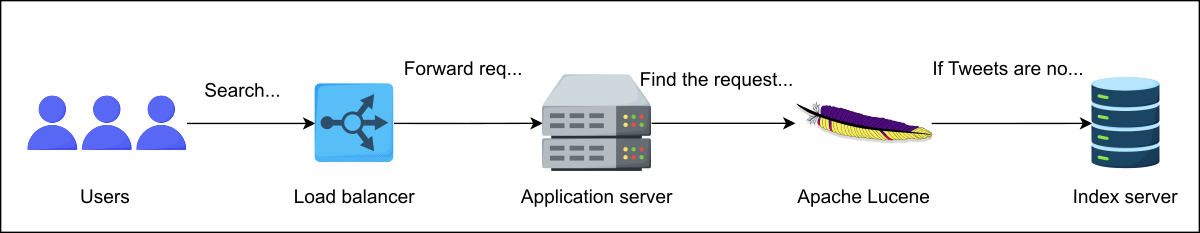
\includegraphics[width=0.5\textwidth]{Images/chapter_31/section_6156135136755712/6199090348425216.png}
 \caption{Processing the search request}
\end{figure}

The solution based on the "one size fits all" approach is infrequently effective. Real -time applications always focus on providing the right tool for the job, which needs to understand all possible use cases. Lastly
, everything has upsides and downsides and should be applied with a sense of reality.

\subsection{Cache}\label{6TuqLvsx9ZxBNbs7Jkl2V}
\\
As we know, caches help to reduce the latency and increase the throughput. Caching is mainly utilized for storage (heavy read traffic), computation (real-time stream processing and machine learning), and transient data (rate limiters). Twitter has been using multi-tenant (multiple instances of an application have a shared environment) Twitter Memcached (Twemcache) and Redis (Nighthawk) clusters for caching. Due to some issues such as unexpected performance, debugging difficulties, and other operational hassles in the existing cache system (Twemcache and Nighthawk), Twitter has started to use the \textbf{Pelikan} cache. This cache gives high-throughput and low latency. Pelikan uses many types of back-end servers such as the peliken\_twemcache replacement of Twitter's Twemcache server, the peliken\_slimcache replacement of Twitter's Memcached/Redis server, and so on. To dive deep, we have a detailed chapter on an \href{https://www.educative.io/courses/grokking-the-system-design-interview/system-design-the-distributed-cache}{In-memory Cache}. Let's have a look at the below illustration representing the relationship of application servers with distributed Pelikan cache.

\begin{figure}[htbp]
 \centering
 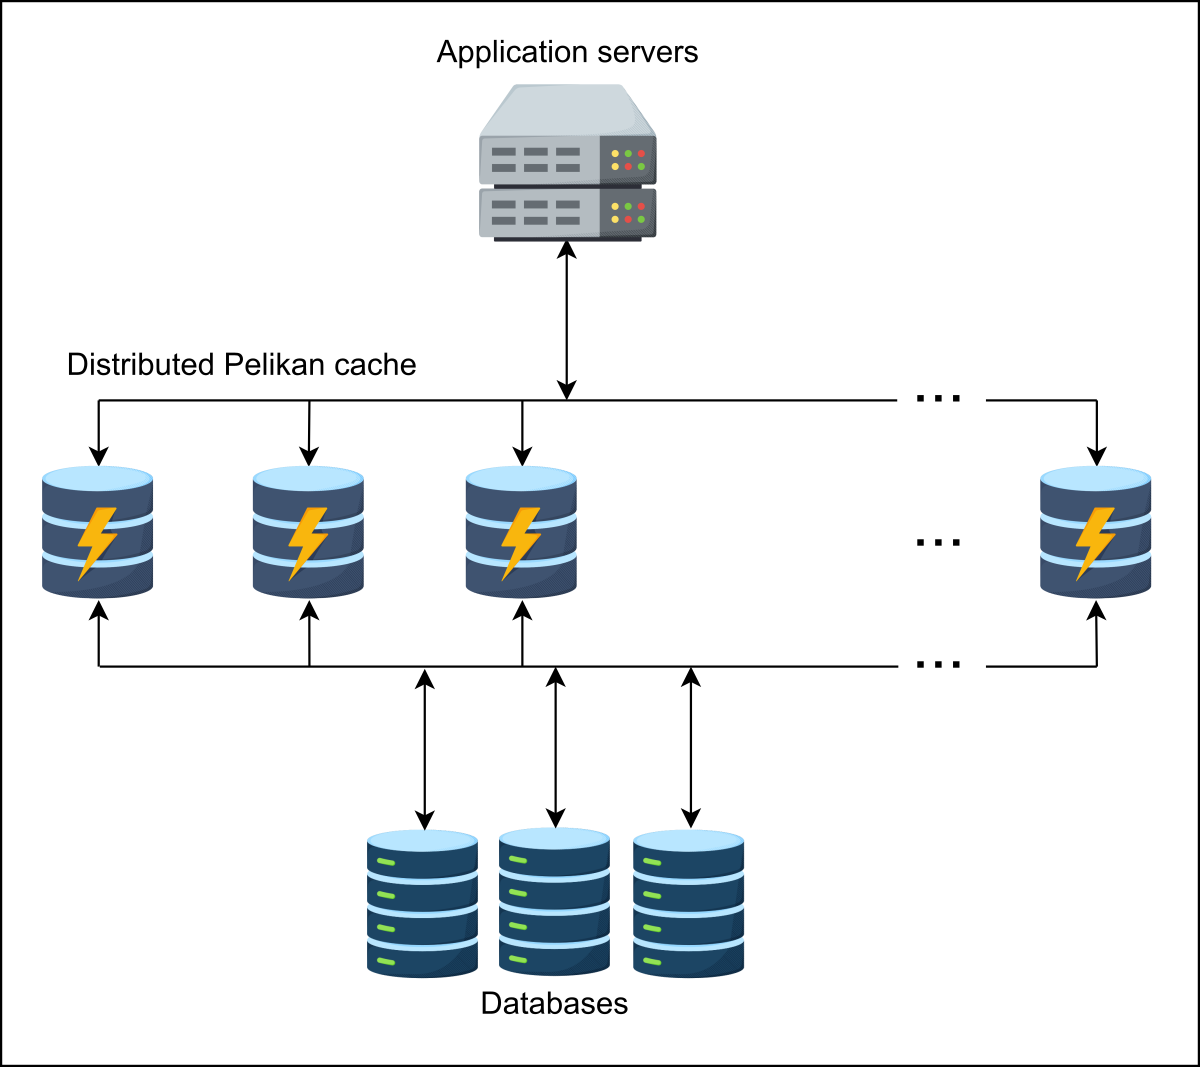
\includegraphics[width=0.5\textwidth]{Images/chapter_31/section_6156135136755712/6076969043492864.png}
 \caption{Distributed Pelikan cache}
\end{figure}

\begin{quote}
\textbf{Note:} Pelikan also introduced another back-end server named \textbf{Segcache}, which is extremely scalable and memory-efficient for small objects. Typically, the median size of the small object is between 200 to 300 bytes in a large-scale application's cache. Most solutions (Memcache and Redis) have a high size (56 bytes) of metadata with each object. This signifies that the metadata takes up more than one-third of the memory. Pelikan reduced metadata size per object to 38 bytes. Segcache also received the NSDI Community Award and is used as an experimental server as of 2021.
\end{quote}

\subsection{Observability}\label{jntc4QKT1yQ0xW0Xvf_dW}
\\
Real-time applications use thousands of servers that provide multiple services. Monitoring resources and their communication inside or outside the system is complex. We can use various tools to monitor services' health, such as providing alerts and support for multiple issues. Our alert system notifies of broken or degraded services triggered by the set metrics. We can also use the dynamic configuration library that deploys and updates the configuration for multiple services without restarting the service. This library leverages the ZooKeeper (discussed later) for the configuration as a source of truth. Twitter used the Loglens service that delivers visualization and analytics of service logs. Later , it was replaced by Splunk Enterprise, a central logging system.
\\
Tracing billions of requests is challenging in large-scale real-time applications. Twitter uses Zipkin, a distributed tracing system, to trace each request (spent time and request count) for multiple services. Zipkin selects a portion of all the requests and attaches a lightweight trace identifier. This sampling also reduces the tracing overhead. Zipkin receives data through the \textbf{Scribe} (real-time log data aggregation) server and stores it in the key-value stores with few indexes.

\begin{figure}[htbp]
 \centering
 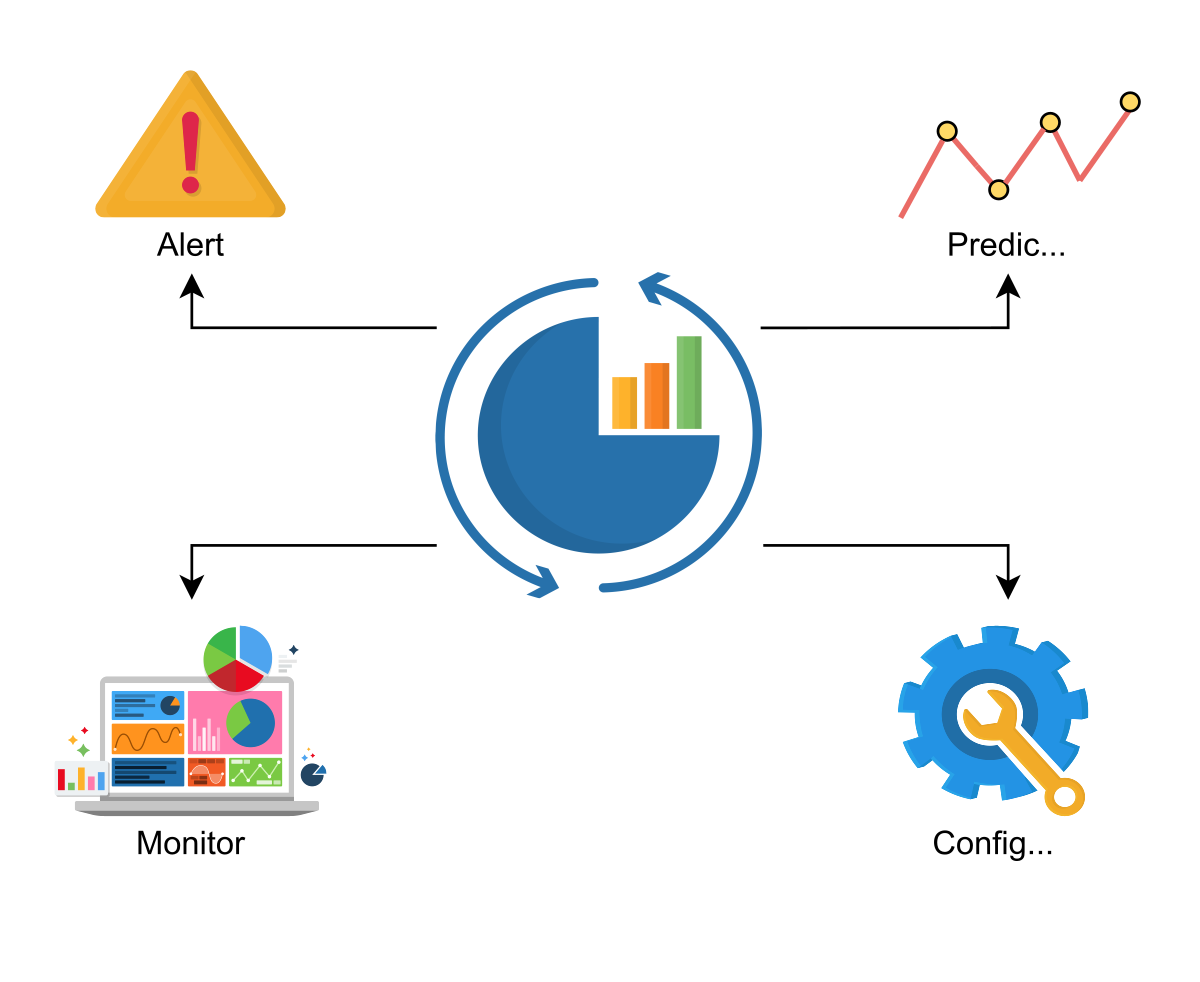
\includegraphics[width=0.5\textwidth]{Images/chapter_31/section_6156135136755712/5794214687014912.png}
 \caption{Observability}
\end{figure}

Most real-time applications use ZooKeeper to store critical data. It can also provide multiple services, such as distributed locking and leader election in the distribution system. Twitter uses ZooKeeper to store service registry, Manhattan clusters' topology information, metadata, and so on. Twitter also uses it for the leader election on the various systems.

\subsection{Real-world complex problems}\label{pVzYJ-67jdkbnOOJ0i6Y5}
\\
Twitter has millions of accounts, and some accounts (public figures) have millions of followers. When these accounts post Tweets, millions of followers of the respective account engage with their Tweets in a short time. The problem becomes big when the system handles the billions of interactions (such as views and likes) on these Tweets. This problem is also known as the \textbf{heavy hitter} problem. For this, we need millions of counters to count various operations on Tweets.
\\
Moreover, a single counter for each specific operation on the particular Tweet is not enough. It's challenging to handle millions of increments or decrements requests against a particular Tweet in a single counter. Therefore, we need multiple distributed counters to manage burst write requests (increments or decrements) against various interactions on celebrities' Tweets. Each counter has several shards working on different computational units. These distributed counters are known as \textbf{sharded counters}. These counters also help in another real-time problem named the \textbf{Top-k} problem. Let's discuss an example of Twitter's Top-k problems: trends and timeline.
\\
\textbf{Trends}: Twitter shows Top-k trends (hashtags or keywords) locally and globally. Here, ``locally'' refers to when a topic or hashtag is used within the exact location where the requested user is active. Alternatively, ``globally'' refers to when the particular hashtag is used worldwide. There is a possibility that users from some regions are not using a specific hashtag in their Tweets but get this hashtag in their trends timeline. Hashtags with the maximum frequency (counts) become trends both locally and globally. Furthermore, Twitter shows various promoted trends (known as ``paid trends'') in specified regions under trends. The slides below represent hashtags in the sliding window selected as Top-k trends over time.

\begin{figure}[htbp]
 \centering
 \begin{subfigure}[b]{0.48\textwidth}
 \centering
 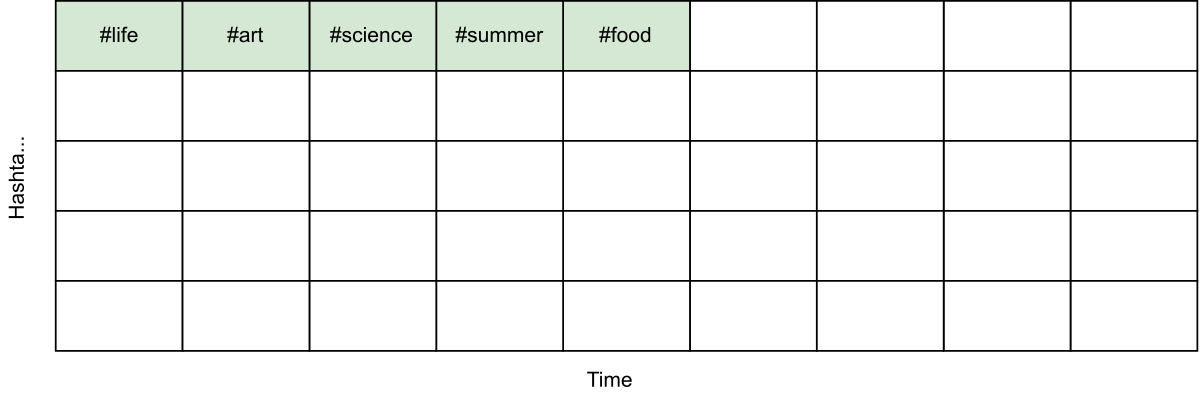
\includegraphics[width=\textwidth]{Images/chapter_31/section_6156135136755712/5710316792446976.png}
 \caption{Top-k trends in a specified time frame}
 \end{subfigure}
 \hfill
 \begin{subfigure}[b]{0.48\textwidth}
 \centering
 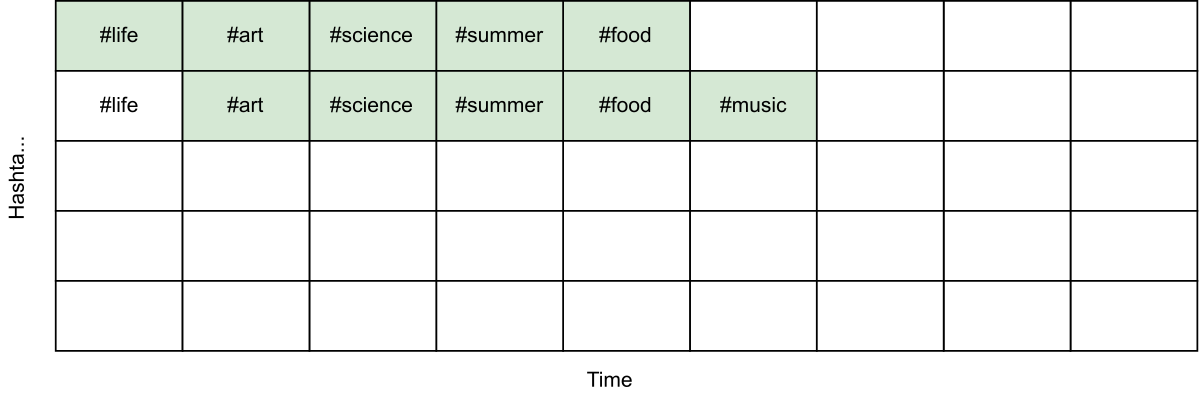
\includegraphics[width=\textwidth]{Images/chapter_31/section_6156135136755712/5965403490091008.png}
 \caption{Dropped \#life hashtag and showing next top-k trends in a specified time frame}
 \end{subfigure}
\end{figure}

\begin{figure}[htbp]
 \centering
 \begin{subfigure}[b]{0.48\textwidth}
 \centering
 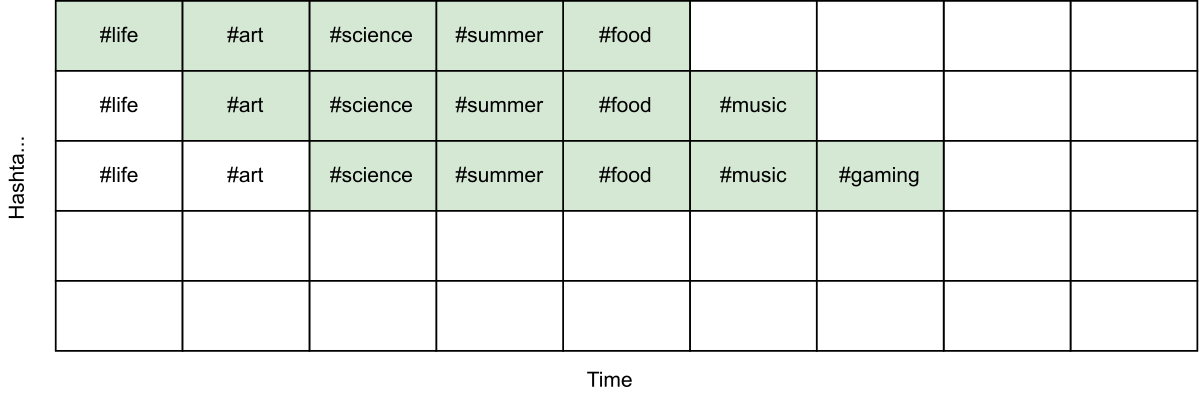
\includegraphics[width=\textwidth]{Images/chapter_31/section_6156135136755712/4839503583248384.png}
 \caption{Dropped \#life and \#art hashtags and showing next top-k trends in a specified time frame}
 \end{subfigure}
 \hfill
 \begin{subfigure}[b]{0.48\textwidth}
 \centering
 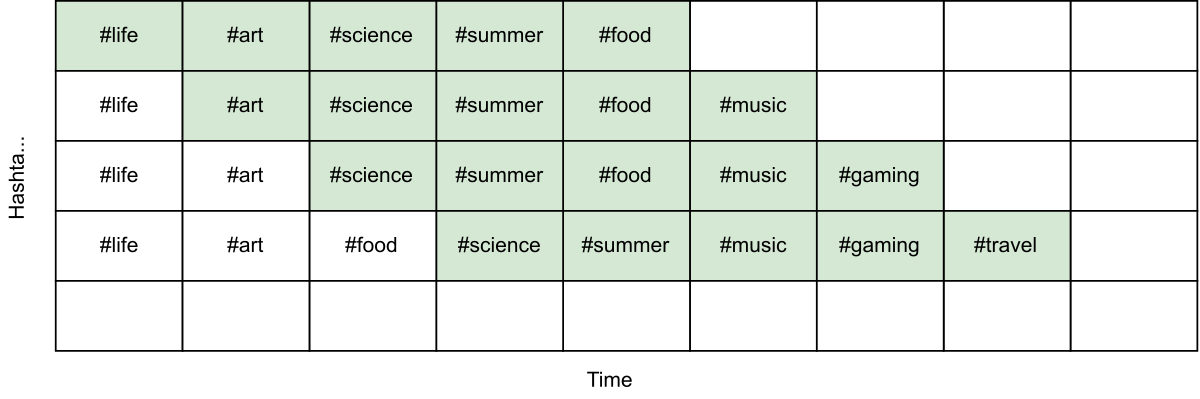
\includegraphics[width=\textwidth]{Images/chapter_31/section_6156135136755712/5683928513380352.png}
 \caption{Dropped \#life, \#art, and \#food hashtags and showing next top-k trends in a specified time frame}
 \end{subfigure}
\end{figure}

\begin{figure}[htbp]
 \centering
 \begin{subfigure}[b]{0.48\textwidth}
 \centering
 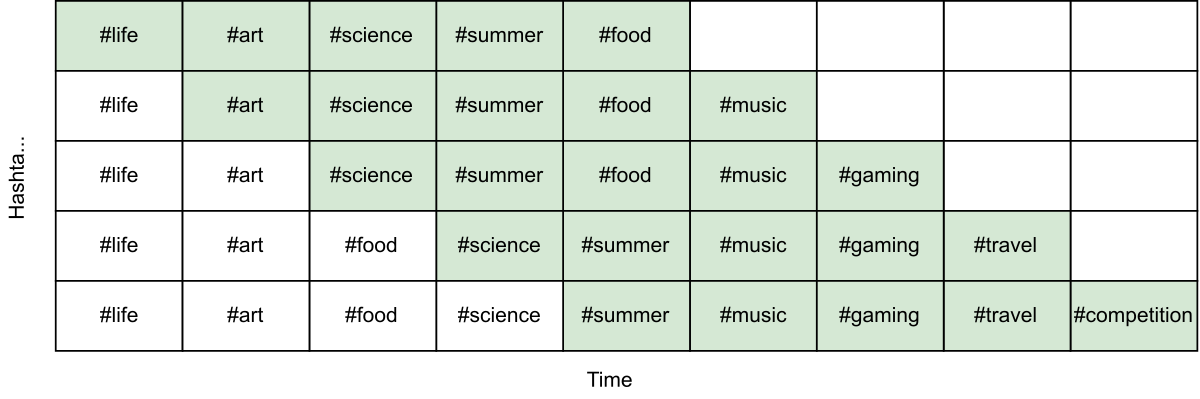
\includegraphics[width=\textwidth]{Images/chapter_31/section_6156135136755712/5991791769157632.png}
 \caption{Dropped \#life, \#art, \#food, and \#science hashtags and showing next top-k trends in a specified time frame}
 \end{subfigure}
\end{figure}

\textbf{Timeline}: Twitter shows two types of timelines: home and user timelines. Here, we'll discuss the home timeline that displays a stream of Tweets posted by the followed accounts. The decision to show Top-k Tweets in the timeline includes followed accounts\textquotesingle{} Tweets and Tweets that are liked or retweeted by the followed accounts. There's also another category of promoted Tweets displayed in the home timeline.
\\
Sharded counters solve the discussed problems efficiently. We can also place shards of the specified counter near the user to reduce latency and increase overall performance like \textbf{CDN}. Another benefit we can get is a frequent response to the users when they interact (like or view) with a Tweet. The nearest servers managing various shards of the respective counters are continuously updating the like or view counts with short refresh intervals. We should note, however, that the near real-time counts will update on the Tweets with a long refresh interval. The reason is the application server waits for multiple counts submitted by the various servers placed in different regions. We have a detailed chapter on \href{https://www.educative.io/courses/grokking-the-system-design-interview/system-design-the-sharded-counters}{Sharded Counters}, explaining how it works in real-time applications.

\subsection{The complete design overview}\label{sPSJCPiUm_7Cr-_cl6Hj_}
\\
This section will discuss what happens in the back-end system when the end users generate multiple requests. The following are the steps:

\begin{itemize}
\item
\protect\phantomsection\label{SixhDIW7q-S2FH1orDNGA}
First, end users get the address of the nearest load balancer from the local DNS.
\item
\protect\phantomsection\label{V_xrW_1cM2XESUhBc2PBk}
Load balancer routes end users' requests to the appropriate servers according to the requested services. Here , we'll discuss the Tweet, timeline, and search services.

\begin{itemize}
\item
\textbf{Tweet service}: When end users perform any operation, such as posting a Tweet or liking other Tweets, the load balancers forward these requests to the server handling the Tweet service. Consider an example where users post Tweets on Twitter using the \texttt{/postTweet} API. The server (Tweet service) receives the requests and performs multiple operations. It identifies the attachments (image, video) in the Tweet and stores them in the Blobstore. Text in the Tweets, user information, and all metadata are stored in the different databases (Manhattan, MySQL, PostgreSQL, Vertica). Meanwhile, real-time processing, such as pulling Tweets, user interactions data, and many other metrics from the real-time streams and client logs, is achieved in the Apache Kafka.\\
Later, the data is moved to the cloud pub-sub through an event processor. Next , data is transferred for deduping(Removal of redundant data) and aggregation to the BigQuery through Cloud Dataflow. Finally
, data is stored in the Google Cloud Bigtable, which is fully managed, easily scalable, and sorted keys.
\item
\textbf{Timeline service}: Assume the user sends a home timeline request using the /viewHome\_timeline API. In this case, the request is forwarded to the nearest CDN containing static data. If the requested data is not found, it's sent to the server providing timeline services. This service fetches data from different databases or stores and returns the Top-k Tweets. This service collects various interactions counts of Tweets from different sharded counters to decide the Top-k Tweets. In a similar way, we will obtain the Top-k trends attached in the response to the timeline request.
\item
\textbf{Search service}: When users type any keyword(s) in the search bar on Twitter, the search request is forwarded to the respective server using the \texttt{/searchTweet} API. It first looks into the RAM in Apache Lucene to get real-time Tweets (Tweets that have been published recently). Then, this server looks up in the index server and finds all Tweets that contain the requested keyword(s). Next, it considers multiple factors, such as time, or location, to rank the discovered Tweets. In the end, it returns the top Tweets.
\end{itemize}
\item
\protect\phantomsection\label{b_3FcnXCydTQk6LnXeCgF}
We can use the Zipkin tracing system that performs sampling on requests. Moreover , we can use ZooKeeper to maintain different data, including configuration information, distributed synchronization, naming registry, and so on.
\end{itemize}

\begin{figure}[htbp]
 \centering
 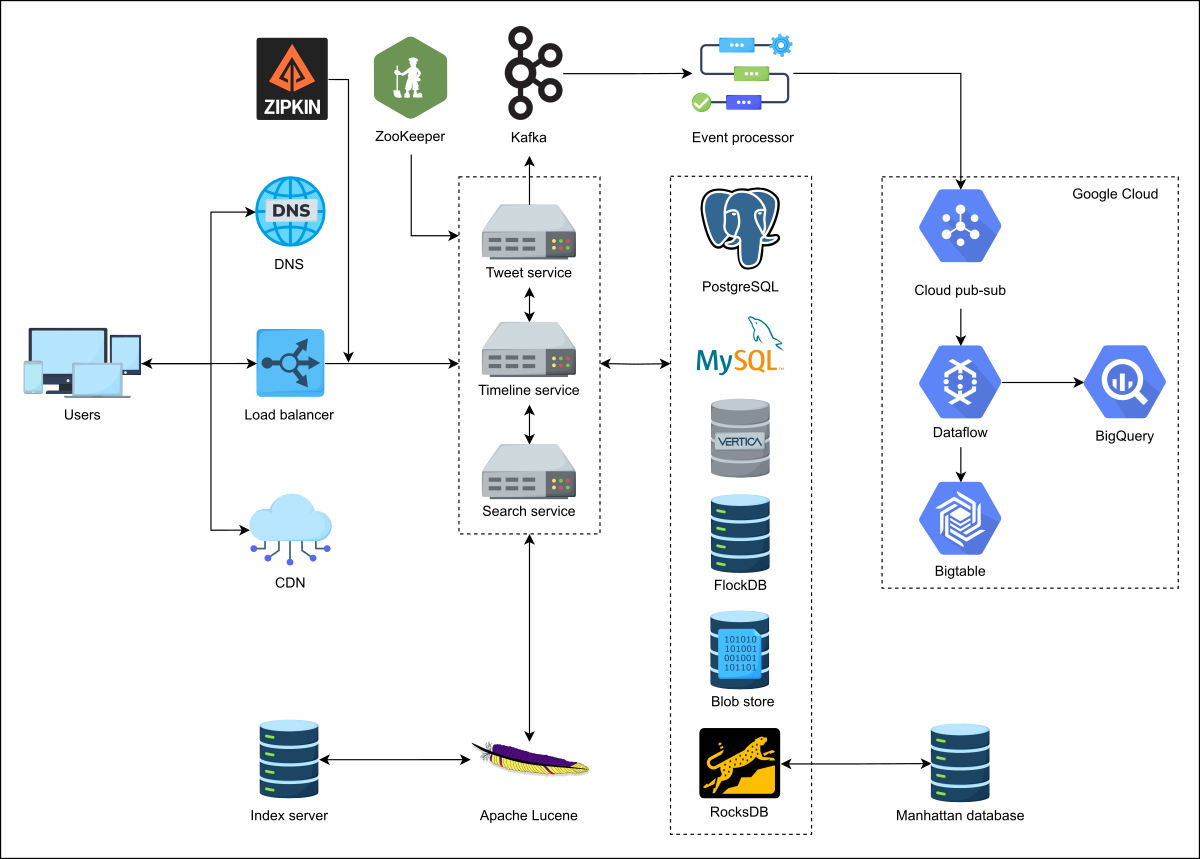
\includegraphics[width=0.5\textwidth]{Images/chapter_31/section_6156135136755712/4972489145188352.png}
 \caption{Twitter design overview}
\end{figure}



% End of section content